\documentclass[acmtog, authorversion]{acmart}

\usepackage{booktabs} % For formal tables

% TOG prefers author-name bib system with square brackets
\citestyle{acmauthoryear}
\setcitestyle{square}

% Copyright
%\setcopyright{acmcopyright}
%\setcopyright{acmlicensed}
%\setcopyright{rightsretained}
%\setcopyright{usgov}
\setcopyright{usgovmixed}
%\setcopyright{cagov}
%\setcopyright{cagovmixed}



% Document starts
\begin{document}
% Title portion
\title{A Neural Network Approach to Stock Prediction}

\author{Paul Soma}
\affiliation{%
  \institution{Michigan State University}}
\email{somapaul@msu.edu}


\maketitle


\section{Introduction}
Accurately forecasting financial markets has been studied extensively by retail traders, investors, and financial institutions the world over. This work employs two neural-network approaches to predicting price action on the Dow Jones Industrial Average.
The Dow Jones Industrial Average (DJI) is a stock market index composed of 30 large publicly traded companies in the United States. The price of the DJI is given by the sum of the price of one share of stock for each of its 30 constituent companies\cite{economics}.

\section{Data}
The data to be studied contains the daily high price, low price, opening price, and closing price, for the DJI from the beginning of January, 2018 through then end of September, 2018. The training set consists of data from Jan 2, 2018 through July 31, 2018, while the test contains set contains data August 1, 2018 through September 28, 2018. Thus the training set consists of 146 days, while the test set consists of 41 days. The validation set consists of 20\% of the data in the training set.

\section{Methods}
This work employs a neural network-based regression approach to predicting price action on the Dow Jones Industrial Average. The data to be studied will contain daily measurements of the DJIA from January through September 2018. Two different approaches were used to predict the DJI. Both approaches utilize artificial neural networks. The difference between the two approaches is that the first approach applied a simple neural network model, while the second approach applied a deep learning model. The differences between the two networks will be covered later in the paper.

\subsection{Data Collection and Preprocessing}
The data was downloaded from Yahoo Finance. A few examples from the data are shown in Table 1. The data was normalized using min-max scaling. The operation for min-max scaling is given in the following equation:
\begin{gather}
    x' = \frac{x - \min x}{\max x - \min x}
\end{gather}
The target variable for each day $t$ in the data was the closing price on the day $t+1$.

\begin{table}[h]
\centering
\caption{Data Features}
\begin{tabular}{p{2.5cm}p{4cm}}

\toprule
\multicolumn{1}{c}{\textbf{Feature}} & \multicolumn{1}{c}{\textbf{Description}}                  \\ \midrule
Open                           & Value at the start of the day         \\
High                           & Highest value of day      \\
Low                           & Lowest value of the day                                     \\
Close                           & Value at the end of the day               \\
Volume                          & Number of shares traded in the day        \\ \bottomrule
\end{tabular}
\end{table}


\begin{table}[]
\centering
\caption{Example Data}
\begin{tabular}{@{}lllll@{}}
\toprule
\textbf{Open} & \textbf{High} & \textbf{Low} & \textbf{Close} & \textbf{Volume} \\ \midrule
22423.47 & 22559.38 & 22416.00 & 22557.59 & 268530000              \\
22564.44 & 22646.32 & 22562.90 & 22641.66 & 238830000              \\
22645.66 & 22685.93 & 22632.80 & 22661.64 & 235730000 \\ \bottomrule
\end{tabular}
\end{table}

\subsection{Model 1}
The architecture of the neural network for model one consisted of 2 hidden layers with 64 and 32 nodes respectively. For the activation function, rectified linear unit is used in both layers. The rectified linear unit (ReLU) is generally a common choice for activation functions for neural networks. The computation of rectified linear unit is shown by equation (2). Mean absolute error was used as the loss function. The network was trained on 1000 epochs. Each epoch represents an iteration of training the model through the entire test set. The model was evaluated using mean absolute error and mean squared error.

\begin{gather}
    ReLU = \max(0,x)
\end{gather}

\subsection{Model 2}
In the model 2 regression approach, the target variable for each $x_t$ is the closing price of $x_{t+1}$. The architecture of the neural network consisted of 5 hidden layers with 128, 64, 32, 16, and 8 nodes respectively. Rectified linear unit is used as the activation function for each layer. Batch normalization is applied after each layer to improve training speed and combat over-fitting. Mean absolute error was used as the loss function. The network was trained on 1000 epochs. The model was evaluated using mean absolute error and mean squared error.

\section{Results}

\subsection{Model 1}
Mean absolute error for model 1 on the training and validation sets are shown in Figure 1. On the test set, model 1 reported a loss of 0.0906, a mean squared error of 0.0106. The actual price and the predicted by the model are shown in Figure 2. In U.S. dollars, the average error for the test set predictions was \$279.55.

\begin{figure}[h]
\caption{Model 1 MAE}
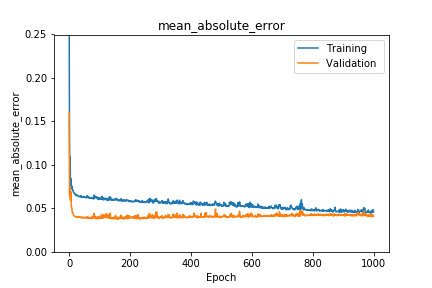
\includegraphics[scale=0.4]{images/model_1_mae.png}
\centering
\end{figure}

\begin{figure}[h]
\caption{Model 1 Prediction}
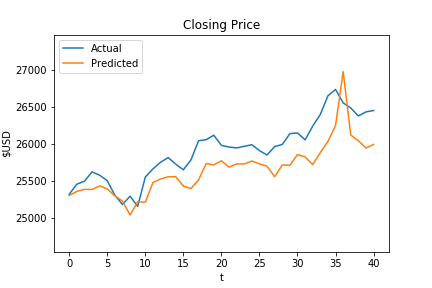
\includegraphics[scale=0.4]{images/model_1_pred.png}
\centering
\end{figure}

\subsection{Model 2}
Mean absolute error for model 2 on the training and validation sets are shown in Figure 3. On the test set, the model 2 reported a loss of 0.0588, a mean squared error of 0.00655, and a mean absolute error of 0.0588. The actual price and the predicted by the model are shown in Figure 2. The average error in U.S. dollars was \$181.46.

\begin{figure}[h]
\caption{Model 2 MAE}
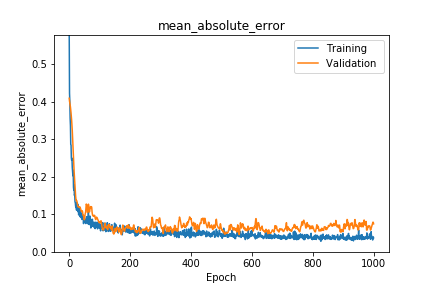
\includegraphics[scale=0.4]{images/model_2_mean_absolute_error.png}
\centering
\end{figure}

\begin{figure}[h]
\caption{Model 2 Prediction}
\includegraphics[scale=0.4]{images/model_2_closing_price.png}
\centering
\end{figure}

\section{Conclusion}
Model 1 suffers from over-fitting. As can be seen from the loss function shown in Figure 1, the validation set has a lower loss than the test set, which should not be the case. Also, the mean absolute error was reduced to 0.0106. We should expect a somewhat higher error. When considering the predicted price shown in Figure 2, we see that the prediction closely mirrors the actual price, but with a large error. This is a sign of overfitting. \\

Model 2 is somewhat more successful than model 1 in that it has less overfitting, likely due to the batch normalization. The price predictions generated by this model are more accurate than the predictions of model 1. However, this model would not be sufficient for use as an actual trading strategy. Future improvements could include trying different activation and loss functions, adding in some computed technical indicators, or using shorter time intervals than 1 day between each record.

\bibliographystyle{plain}
\bibliography{bibliography}


\end{document}
